\documentclass[a4paper]{article}
\usepackage{amsmath}
\usepackage{amssymb}
\usepackage{enumerate}
\usepackage[normalem]{ulem}
\usepackage{cancel}
\usepackage{physics}
\usepackage{hyperref}
\usepackage{graphicx}
\graphicspath{ {./img/} }
\begin{document}
    \subsubsection*{Access Jupyter notebook file in \href{run:../Answere/JupyterNotebook/}{here}, best run using jupyter notebook or using VSCode}
    \begin{enumerate}
        \item $b = [0.4,0.65,0.21,0.61]$
        \item $b = [0.924,0,0,0.383]$
        \item 2 qubit placed in a superposition
        \item 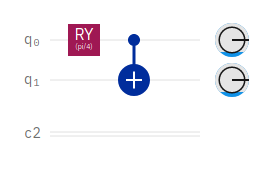
\includegraphics{circuit-klnnmbgw.png}
        \item $\bra{\Psi^{+}}\hspace{2px}(psi^{+})$
        \item $\bra{\Phi^{-}}\hspace{2px}(phi^{-})$
    \end{enumerate}
This document write using \LaTeX \ author: Felix Montalfu(03082180055)
\end{document}